\documentclass[12pt,a4paper]{article}
\usepackage[centertags]{amsmath}
\usepackage{graphicx}
\usepackage{caption3}
\usepackage{misccorr}
\usepackage{epsfig}
\usepackage{indentfirst}
\usepackage{ulem}
\usepackage[utf8]{inputenc}
\usepackage[english, russian]{babel}
\usepackage{setspace}
\usepackage{amssymb,amsfonts,amsmath,mathtext,braket,stmaryrd,mathrsfs}
\usepackage{cite}
\usepackage{subfigure}
\bibliographystyle{iopart-num}
\usepackage{geometry} % пакет для задания полей страницы командой \geometry
\geometry{left=3cm,right=1.5cm,top=2cm,bottom=2cm}
\numberwithin{equation}{section}
\DeclareMathOperator{\sign}{sign}
\DeclareMathOperator{\rot}{rot}
\DeclareMathOperator{\diver}{div}
\DeclareMathOperator{\w}{w}
\DeclareMathOperator{\Q}{Q}
\DeclareMathOperator{\Z}{Z}
\DeclareMathOperator{\F}{F}
\DeclareMathOperator{\M}{M}
\DeclareMathOperator{\q}{q}
\DeclareMathOperator{\g}{g}
\DeclareMathOperator{\h}{h}
\DeclareMathOperator{\e}{e}
\DeclareMathOperator{\vp}{\mathbf {v.p.}}
\makeatletter
\renewcommand \thesection {\@arabic\c@section}
\renewcommand\thesubsection {\thesection.\@arabic\c@subsection}
\renewcommand{\theequation}{\thesection.\arabic{equation}}
%\renewcommand{\thefigure}{\thesection.\arabic{figure}}
\linespread{1.3} % полтора интервала. Если 1.6, то два интервала
\renewcommand{\appendix}{\setcounter{section}{0}\gdef\thesection{\@Alph\c@section}}


\pagestyle{plain}

\begin{document}
\section{Особенности фотоэлектронов в плазме инертных газов}
Рассмотрим плазму, образованную при ионизации атомов инертных газов коротким импульсом лазерного излучения (см., например, \cite{refAGOSTINI1,refAGOSTINI2,refPOPOV}). Согласно теории Келдыша, режим многофотонной ионизации реализуется при достаточно низкой интенсивности ионизующего излучения. В этом случае распределение фотоэлектронов по энергиям имеет вид узкого пика, отвечающего поглощению минимально необходимого количества фотонов для преодоления порога ионизации, определяющегося потенциалом ионизации атома $E_i$. Положение максимума функции распределения фотоэлектронов соответствует энергии $\epsilon_0$, определяемой согласно формуле многофотонного фотоэффекта $\epsilon_0=K\hbar\Omega-E_i$ и имеющей значение порядка нескольких $eV$. Здесь $\hbar$ - постоянная Планка, $\Omega$ - частота ионизирующего излучения.

Вообще говоря, это распределение является анизотропным, однако если плазма является слабоионизованной, то рассеяние фотоэлектронов на нейтральных атомах приводит к быстрой релаксации направления их скоростей. Рассмотрим времена, превышающие обратную эффективную частоту упругих столкновений фотоэлектронов и для описания распределения фотоэлектронов по скоростям воспользуемся изотропной функцией, которая остается неравновесной и отвечает пикообразному энергетическому спектру. Будем считать разбросом скоростей несущественным и используем функцию распределения, отвечающую модели ''холодной'' плазмы
\begin{equation}
\label{FR}
f\left(v\right)=\frac{n}{4\pi v_0^2}\, \delta\left(v-v_0\right),
\end{equation}	
где $n$ - плотность фотоэлектронов, $v_0 = \sqrt{2\epsilon_0/m}$, $m$ — масса электрона. Неравновесное распределение \eqref{FR} релаксирует к распределению Максвелла из-за электрон-электронных столкновений и квазиупругих столкновений фотоэлектронов с нейтральными атомами на существенно больших временах. Ниже будем рассматривать воздействие излучения, частота которого много больше, чем характерные обратные времена релаксации функции \eqref{FR}.

Отметим, что при многофотонной ионизации типичная энергия $\epsilon_0$ не превышает нескольких $eV$. В случае одноатомных инертных газов нижний порог возбуждения внутриатомных электронных состояний при столкновениях электронов и атомов заметно выше. Например, для атома $\textrm{Xe}$ такой порог превышает $8 \text{eV}$, а для атомов криптона  -- $10 \text{eV}$. Поэтому рассеяние фотоэлектронов определяется в основном упругими столкновениями с нейтральными атомами. Ниже будем использовать частоту столкновений фотоэлектронов с нейтральными атомами, которая определяется как $\nu\left(v\right)= N\sigma_{tr}\left(v\right)v$, где $N$ - концентрация нейтральных атомов, $\sigma_{tr}\left(v\right)$ - транспортное сечение рассеяния электронов на нейтральных атомах, которое зависит от скорости фотоэлектронов. Слабоионизованность плазмы позволяет считать концентрацию нейтральных атомов постоянной величиной. Также  учтем, что в инертных газах транспортное сечение рассеяния в области энергий чуть меньших $1\text{eV}$ имеет минимум \cite{refTOWNSEND, refRAMSAUER,refBRODE} и в точке, отвечающей средней энергии фотоэлектронов, имеет положительную производную.   

%Используя значения транспортного сечения упругого рассеяния электронов на атомах $\textrm{Xe}$, приведенные в \cite{refXe2}, для $\nu\left(v\right)$ имеем зависимость, представленную на рис. \ref{nu_xe}. Точки на кривой рис. \ref{nu_xe} отвечают экспериментальным данным работы \cite{refXe2}. Аналогичная зависимость частоты столкновений от энергии при рассеянии фотоэлектронов на атомах криптона приведена на рис. \ref{nu_kr}. 
%Экспериментальные данные для криптона взяты из работы \cite{refPACK}. В
%ксеноне частота столкновений возрастает в диапазоне энергий $\epsilon \sim \left(0.6\div\, 6\right)\, eV$, а в криптоне – в диапазоне $\epsilon \sim \left( 0.5 \div\, 10 \right)\, eV$. В дальнейшем будет показано, что наличие такого участка отвечает за усиление поглощения падающей электромагнитной волны.

\section{Постановка задачи}
Рассмотрим проникновение H-волны в неоднородную холодную плазму, образованную при многофотонной ионизации инертных газов. Выберем систему координат таким образом, что падающая электромагнитная волна имеет вид $\bm{E}\left(z,t\right) =(1/2)\left(E_0,0,0\right)\cdot\exp\left[-i\omega\left(t-z/c\right)\right]+c.c.$, где. $c$ -- скорость света,  $\omega$ -- частота. Фотоионизованная плазма занимает полупространство $z>0$ и имеет распределение фотоэлектронов вида \eqref{FR}. При этом плотность плазмы $n\to 0$ при $z\to0$ и линейно возрастает до величины $n\left(L\right) = n_0$, после чего при $z>L$ остается постоянной.  Электромагнитная волна порождает в плазме направленное вдоль оси $ox$ электрическое поле вида $(1/2)\bm{E}\left(z\right)\cdot\exp\left(-i\omega t\right)+c.c.$ и приводит к малому возмущению функции распределения фотоэлектронов по скоростям вида $(1/2)\,\delta f(\mathbf v,z)\exp\left(-i\omega t\right)+c.c$. Рассмотрим случай, когда частота падающей электромагнитной волны достаточно велика $$ \frac{v_0}{c}\ll \frac{\omega}{\omega_L}.$$ В этом случае дисперсионными поправками можно пренебречь. Поэтому для определения $\delta f\left(\mathbf v,z\right)$ воспользуемся следующим линеаризованным кинетическим уравнением с интегралом столкновений, описывающим релаксацию по направлениям скорости фотоэлектронов без изменения их энергии,
\begin{equation}
\label{kinetic}
    -i\omega\delta f(\mathbf v,z)+\frac{ev_x E\left(z\right)}{mv}\frac{\partial f_0(v, z)}{\partial v}= -\nu\left(v\right) \left[\delta f(\mathbf v,z)-\int \frac{d\Omega}{4\pi}\delta f(\mathbf v,z)\right],
\end{equation}
где $e$ — заряд электрона, $d\Omega$ -- элемент телесного угла.
Для определения поля в плазме воспользуемся самосогласованной системой уравнений Максвелла и уравнения \eqref{kinetic}. Тогда получим
\begin{equation}
    \label{field}
    \frac{d^2E}{dz^2}+\frac{\omega^2}{c^2}E = -\frac{4\pi i \omega}{c^2}j,
\end{equation}
где выражение для плотности тока в плазме с учетом зависимости частоты столкновений фотоэлектронов от их скорости имеет вид
\begin{equation}
    \label{current}
    j = \frac{e^2}{m} \int d\bm{v} \frac{v_x^2}{v}\frac{\partial f_0}{\partial v} \frac{E\left(z\right)}{i\omega-\nu\left(v\right)}.
\end{equation}
Вычислив интеграл в выражении для плотности тока \eqref{current}, уравнение \eqref{field} можно переписать в виде
\begin{equation}
    \label{field2}
    \frac{d^2E}{dz^2}+\frac{\omega^2}{c^2}\varepsilon\left(\omega, z\right)E = 0,
\end{equation}
где диэлектрическая проницаемость имеет вид
\begin{equation}
    \label{perm_fin}
    \varepsilon(\omega, z)=1-\frac{\omega_L^2\left(z\right)}{\omega\left(\omega+i\nu\right) }\left[1-i\frac{\alpha}{3}\frac{\nu}{\omega+i\nu}\right].
\end{equation}
Здесь $\omega_L\left(z\right) = \sqrt{4\pi n\left(z\right)e^2/m}$ — ленгмюровская частота электронов, $\nu\equiv\nu\left(v_0\right),\alpha=\partial \ln\nu/\partial \ln v_0%|_{v = v_0}%
$ — величина, определяющаяся средней энергией фотоэлектронов и видом зависимости транспортного сечения рассеяния от энергии. %Поскольку плотность электронов является линейной функцией координаты, то уравнение \eqref{field2} подстановкой 
%\begin{equation}
%    \label{xi}
%    \xi = \left(\frac{4\pi \beta e^2\omega}{mc^2\left(\omega+i\nu\right)\left(1-i\alpha/3 \left(\nu/\left(\omega+i\nu\right)\right)\right)^2}\right)^{1/3}\left[\frac{m\omega\left(\omega+i\nu\right)}{4\pi\beta e^2} -z\left(1-i\frac{\alpha}{3}\frac{\nu}{\omega+i\nu}\right)\right]
%\end{equation} может быть приведено к уравнению Эйри
%\begin{equation}
%    \label{Aery}
%    \frac{d^2 E}{d\xi^2}+\xi E = 0.
%\end{equation}
%В \eqref{xi} $\beta$ - коэффициент пропорциональности между плотностью электронов и координатой $z$.
%Решение уравнения \eqref{Aery}, убывающее на бесконечности имеет вид
%\begin{equation}
%    \label{solve}
%    E\left(\xi\right) = \frac{3A}{\pi}\int_{0}^{\infty} \cos\left(\frac{y^3}{3}-\xi y\right)dy,
%\end{equation}
%где коэффициент $A$ определяется из граничных условий.
\section{Общее решение}
Область, занимаемую плазмой, можно разделить на две части, - ту, где плотность электронов меняется линейно и ту, где она является постоянной величиной. В области $0<z<L$ выражение \eqref{perm_fin}} можно переписать в виде 
\begin{equation}
    \label{perm_f}
    \varepsilon(\omega, z) = 1 - \frac{z}{L} \omega_L^2 f\left(\omega, \nu, \alpha\right),
\end{equation}
где $\omega_L \equiv \omega_L\left(L\right)$, а функция 
\begin{equation}
    \label{f}
    f\left(\omega, \nu, \alpha\right) = \frac{1}{\omega\left(\omega+i\nu\right)}\left[1-i\frac{\alpha}{3}\frac{\nu}{\omega+i\nu}\right]
\end{equation}
определяется из соотношений между частотой падающего поля, частотой столкновений фотоэлектронов и параметром $\alpha$. 
Поскольку диэлектрическая проницаемость является линейной функцией координаты, то уравнение \eqref{field2} подстановкой 
\begin{equation}
    \xi = \left(\frac{\omega^2}{z_0 c^2}\right)^{1/3}\left(z-z_0\right)
\end{equation}
может быть приведено к уравнению Эйри
\begin{equation}
    \label{Aery}
    \frac{d^2 E}{d\xi^2}-\xi E = 0,
\end{equation}
где 
\begin{equation}
    z_0 = \frac{1}{f\left(\omega, \nu, \alpha\right)\omega_L^2}L.
\end{equation}
Решением уравнения \eqref{Aery} будет сумма двух функций Эйри  с коэффициентами, определяемыми из граничных условий,
\begin{equation}
    \label{field_L}
    E\left(\xi\right) = C_1 Ai\left(\xi\right)+C_2 Bi\left(\xi\right).
\end{equation}
 

В области $z>L$ плотность электронов постоянна, поэтому диэлектрическая проницаемость перестает зависеть от координаты $z$ и решением уравнения \eqref{field} будет убывающая экспоненциально волна вида
\begin{equation}
    \label{field_inf}
    E\left(z\right) = C_3\exp\left[i\frac{\omega}{c}\sqrt{\varepsilon\left(\omega\right)}z\right],
\end{equation}
где $\varepsilon\left(\omega\right) \equiv \varepsilon\left(\omega, L\right)$, и выбрана ветвь квадратного корня на комплексной плоскости такая, что $\Im \sqrt{\varepsilon\left(\omega\right)}>0$.

Для того, чтобы найти неизвестные коэффициенты $C_1, C_2, C_3$ воспользуемся граничными условиями. На границе плазмы $z=0$ тангенциальные компоненты электрического и магнитного полей непрерывны 
\begin{equation}
\label{bound}
    E_0+E_r=E(+0), \qquad  E_0-E_r=B(+0),
\end{equation}
где $E_r$ - амплитуда волны, уходящей от границы плазмы в область $z<0$. Аналогично и при $z=L$ поле и его производные должны быть непрерывными. Таким образом, получаем систему из 4 уравнений на 4 неизвестных.  Обозначим $\xi\left(0\right) = \xi_0, \xi\left(L\right) = \xi_L$.Тогда
\begin{equation}
    \label{system}
    \begin{cases}
    E_0+E_r = C_1 Ai\left(\xi_0\right)+C_2 Bi\left(\xi_0\right), \\
    E_0-E_r=-i\frac{c}{\omega}\left[Ai\,'_z\left(\xi_0\right)+C_2 Bi\,'_z\left(\xi_0\right)\right],\\
    C_1 Ai\left(\xi_L\right)+C_2 Bi\left(\xi_L\right)=C_3\exp\left[i\frac{\omega}{c}\sqrt{\varepsilon\left(\omega\right)} L\right], \\
    C_1 Ai\,'_z\left(\xi_L\right)+C_2 Bi\,'_z\left(\xi_L\right)=  C_3\left(i\frac{\omega}{c}\sqrt{\varepsilon\left(\omega\right)}\right)\exp\left[i\frac{\omega}{c}\sqrt{\varepsilon\left(\omega\right)} L\right].
    
    \end{cases}
\end{equation}

Учтем зависимость $\xi$ от $z$ при взятии производных от функций Эйри
\begin{equation}
    Ai\,'_z\left(\xi\left(z\right)\right) = \left(\frac{\omega^2}{z_0 c^2}\right)^{1/3}Ai\,'\left(\xi\right) \equiv \xi' Ai\,'\left(\xi\right),
\end{equation}
Исключая $E_r$ из первых двух уравнений системы и учитывая связь между коэффициентами $C_1$ и $C_2$, полученную из последних двух уранений системы \eqref{system}, получим для коэффициентов $C_1$ и $C_2$ следующие выражения
\begin{equation}
    \label{C1_common}
    \begin{array}{lcl}
         C_1 = -2E_0\left[-i\frac{\omega}{c}Bi\left(\xi_L\right)\sqrt{\varepsilon\left(\omega\right)}+\xi'Bi\,'\left(\xi_L\right)\right]\times \\
       \left\{\left[Bi\left(\xi_0\right)-i\frac{c}{\omega}\xi'Bi\,'\left(\xi_0\right)\right]\left[-i\frac{\omega}{c}Ai\left(\xi_L\right)\sqrt{\varepsilon\left(\omega\right)}+\xi'Ai\,'\left(\xi_L\right)\right] - \right.\\ 
       \left.\left[Ai\left(\xi_0\right)-i\frac{c}{\omega}\xi'Ai\,'\left(\xi_0\right)\right]\left[-i\frac{\omega}{c}Bi\left(\xi_L\right)\sqrt{\varepsilon\left(\omega\right)}+\xi'Bi\,'\left(\xi_L\right)\right]\right\}^{-1},
    \end{array}
\end{equation}

\begin{equation}
    \label{C2_common}
    \begin{array}{lcl}
         C_2 = 2E_0\left[-i\frac{\omega}{c}Ai\left(\xi_L\right)\sqrt{\varepsilon\left(\omega\right)}+\xi'Ai\,'\left(\xi_L\right)\right]\times \\
       \left\{\left[Bi\left(\xi_0\right)-i\frac{c}{\omega}\xi'Bi\,'\left(\xi_0\right)\right]\left[-i\frac{\omega}{c}Ai\left(\xi_L\right)\sqrt{\varepsilon\left(\omega\right)}+\xi'Ai\,'\left(\xi_L\right)\right] - \right.\\ 
       \left.\left[Ai\left(\xi_0\right)-i\frac{c}{\omega}\xi'Ai\,'\left(\xi_0\right)\right]\left[-i\frac{\omega}{c}Bi\left(\xi_L\right)\sqrt{\varepsilon\left(\omega\right)}+\xi'Bi\,'\left(\xi_L\right)\right]\right\}^{-1}.
    \end{array}
\end{equation}

Определим коэффициент отражения на границе плазмы как
\begin{equation}
    \label{refl}
    R = \frac{E_r}{E_0}.
\end{equation}
Вычислив $E_r$ из системы \eqref{system} и подставляя значения коэффициентов $C_1$ и $C_2$, получим в общем виде выражение для коэффициента отражения
\begin{equation}
\label{coeff}
\begin{array}{lcl}
  R = \left\{\left[Bi\left(\xi_0\right)+i\frac{c}{\omega}\xi'Bi\,'\left(\xi_0\right)\right]\left[-i\frac{\omega}{c}Ai\left(\xi_L\right)+\xi'Ai\,'\left(\xi_L\right)\right] - \right. \\
  \left.\left[Ai\left(\xi_0\right)+i\frac{c}{\omega}\xi'Ai\,'\left(\xi_0\right)\right]\left[-i\frac{\omega}{c}Bi\left(\xi_L\right)\sqrt{\varepsilon\left(\omega\right)}+\xi'Bi\,'\left(\xi_L\right)\right]\right\}\times \\
  \left\{\left[Bi\left(\xi_0\right)-i\frac{c}{\omega}\xi'Bi\,'\left(\xi_0\right)\right]\left[-i\frac{\omega}{c}Ai\left(\xi_L\right)+\xi'Ai\,'\left(\xi_L\right)\right] \right. -\\
   \left.\left[Ai\left(\xi_0\right)-i\frac{c}{\omega}\xi'Ai\,'\left(\xi_0\right)\right]\left[-i\frac{\omega}{c}Bi\left(\xi_L\right)\sqrt{\varepsilon\left(\omega\right)}+\xi'Bi\,'\left(\xi_L\right)\right]\right\}^{-1}.
\end{array}
\end{equation}

Коэффициент поглощения $A\left(\omega\right)$, характеризующий долю переданной плазме энергии падающей волны, имеет вид
\begin{equation}
    \label{absorp_common}
    A\left(\omega\right) = 1-\left|R\right|^2.
\end{equation}
Свойства функций Эйри позволяют написать асимптотические выражения для электрического поля внутри плазмы. В общие выражения для $E\left(z\right)$ и коэффициента поглощения входят значения функций Эйри в точках $\xi_0$ и $\xi_L$, абсолютные значения которых в условиях малости частоты столкновений и частоты падающего поля по сравнению с плазменной частотой $\omega_L$ имеют вид 
\begin{equation}
\label{xi}
    |\xi_0|= \frac{1}{\omega_L^2}\left|\left(\frac{\omega_L}{c}L\frac{\omega}{f}\right)^{2/3}\right|,\quad |\xi_L|\approx \left|\xi_0 \left[f\left(\omega, \nu, \alpha\right)\omega_L^2-1\right]\right| .
\end{equation}
\section{Высокочастотный скин-эффект}
В разреженной плазме частоты столкновений фотоэлектронов сравнительно малы и интерес представляют условия, когда $\omega \gg \nu$. В этом случае функция $f\left(\omega, \nu, \alpha\right)$ \eqref{f} в линейном приближении по $\nu/\omega$ имеет вид
\begin{equation}
    \label{f_hf}
    f\left(\omega, \nu, \alpha\right) \approx \frac{1}{\omega^2}\left[1-i\left(1+\frac{\alpha}{3}\right)\frac{\nu}{\omega}\right].
\end{equation}
Корень из диэлектрической проницаемости в области постоянной плотности фотоэлектронов с учетом выбора знака имеет значение
\begin{equation}
    \label{perm_nu}
    \sqrt{\varepsilon\left(\omega\right)} = i\frac{\sqrt{\omega_L^2-\omega^2}}{\omega}\gamma,
\end{equation}
где $\gamma = 1-i/2\left(1+\alpha/3\right)\omega_L^2\nu/\omega\left(\omega_L^2-\omega^2\right)$.

Абсолютные значения $\xi_0$ и $\xi_L$ с учетом \eqref{f_hf} принимают значения
\begin{equation}
\label{xi_hf}
    |\xi_0|\approx \frac{\omega^2}{\omega_L^2}\left(\frac{\omega_L}{c}L\right)^{2/3},\quad |\xi_L|\approx \left(\frac{\omega_L}{c}L\right)^{2/3}.
\end{equation}
При этом из \eqref{xi_hf}, \eqref{f_hf} и условии, что плазменная частота $\omega_L$ достаточно велика, видно, что $|\xi_0|<|\xi_L|$. Исходя из соотношения между значениями \eqref{xi_hf} и единицей, можно рассмотреть три предельных случая в зависимости от ширины слоя переменной плотности.
\subsection{Случай узкого слоя переменной плотности}
 Рассмотрим случай, когда ширина слоя меньше электромагнитного масштаба
\begin{equation}
    \label{cond1}
    L<\frac{c}{\omega_L}.
\end{equation}
При таком условии $|\xi_L|\ll 1$, а следовательно и $|\xi_0|\ll 1$. Для малых аргументов функций Эйри справедливо следующее асимптотическое разложение [ссылка на Абрамовица]
\begin{equation}
    \label{asymp_small}
    Ai\left(\xi\right) = \frac{1}{3^{2/3}\Gamma\left(2/3\right)}-\frac{1}{3^{1/3}\Gamma\left(1/3\right)}\xi, \quad 
    Bi\left(\xi\right) = \sqrt{3}\left(\frac{1}{3^{2/3}\Gamma\left(2/3\right)}+\frac{1}{3^{1/3}\Gamma\left(1/3\right)}\xi\right).
\end{equation}
Тогда, учитывая значения функций Эйри  \eqref{asymp_small}, имеем выражение для поля внутри слоя переменной плотности 
\begin{equation}
    \label{E1_small}
     E\left(z\right)= 2E_0\frac{\left(L-z\right)\sqrt{\omega_L^2-\omega^2} \gamma/c+1}{\left(L+i\frac{c}{\omega}\right)\frac{\sqrt{\omega_L^2-\omega^2}}{c}\gamma+1}.
\end{equation}
А в области $z>L$ поле имеет вид
\begin{equation}
    \label{E2_small}
     E\left(z\right) = 2E_0   \frac{\exp\left[-\frac{\sqrt{\omega_L^2-\omega^2}}{c}\gamma\left(z-L\right)\right]}{\left(L+i\frac{c}{\omega}\right)\frac{\sqrt{\omega_L^2-\omega^2}}{c}\gamma+1}.
\end{equation}
Таким образом, поле внутри слоя переменной плотности убывает линейно внутрь плазмы, а, когда плотность плазмы становится постоянной, убывает экспоненциальным образом. Точное решение для абсолютного значения поля внутри плазмы $E\left(z\right)$ продемонстрировано на рис.\ref{E_small}. График на рисунке \ref{E_small} построен с использованием общих выражений \eqref{C1_common} и \eqref{C2_common} для параметров $\alpha = 4.8$, что соответствует плазме, полученной при трехфотонной ионизации ксенона со средней энергией фотоэлектронов $\epsilon_0=2.87\text{eV}$ [ссылка на Попова], частоты падающего поля $\omega = 0.5\omega_L$, частоты столкновений фотоэлектронов $\nu = 0.01 \omega_L$ и ширины слоя $L = 1/3 c/\omega_L$. Точками на оси $x$ обозначены характерные масштабы рассматриваемой задачи, и введено обозначени $\delta = c/\omega_L$. Как видно из рисунка \eqref{E_small} поле внутрь плазмы проникает на расстояние порядка нескольких электромагнитных масштабов.
\begin{figure}[!ht]	
	\center{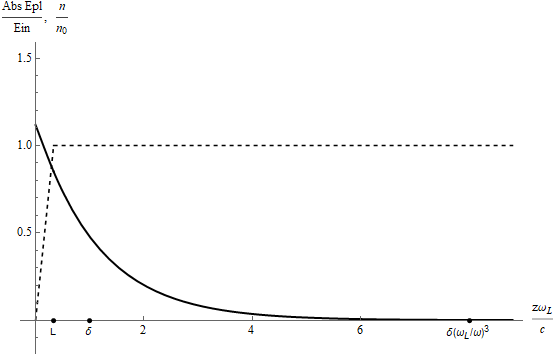
\includegraphics[scale=0.65]{thin_layer.png}}
	\caption{Зависимость абсолютного значения  поля внутри плазмы от расстояния до границы плазмы $z=0$.}
    \label{E_small}
\end{figure}
Из выражения \eqref{coeff} получим коэффициент отражения в виде

\begin{equation}
    \label{coeff1_small}
    R = -\frac{i\sqrt{\omega_L^2-\omega^2}\gamma/\omega - 1}{i\sqrt{\omega_L^2-\omega^2}\gamma/\omega + 1}.
\end{equation}
Тогда, учитывая связь коэффициента отражения с коэффициентом поглощения и подставляя выражение для $\gamma$, имеем
\begin{equation}
\label{coeff2_small}
    A\left(\omega\right) = 2 \frac{\nu}{\sqrt{\omega_L^2-\omega^2}}\left(1+\frac{\alpha}{3}\right).
\end{equation}
Этот же результат получается, если рассматривать плазму с резкой границей, то есть $L \to 0$ [ссылка на нашу работу]. Таким образом, если в плазме, образованной при многофотонной ионизации инертного газа, размытие границы мало по сравнению с электромагнитным масштабом, то границу можно считать резкой.
\subsection{Случай промежуточной ширины слоя}
Поскольку $|\xi_0|<|\xi_L|$, то можно рассмотреть случай, когда $|\xi_0|\ll 1$, а $|\xi_L| \gg 1$. Такие параметры соответсвуют ширине слоя переменной плотности в пределах 
\begin{equation}
    \label{cond2}
    \frac{c}{\omega_L}<L<\frac{\omega_L^3}{\omega^3} \frac{c}{\omega_L}.
\end{equation}
Для больших аргументов функций Эйри имеют место следующие асимптотические выражения [Абрамовиц]
\begin{subequations}
\label{asymp_big}
\begin{align}
    Ai\left(\xi\right) &= \frac{1}{2\sqrt{\pi}\xi^{1/4}}\exp\left[-\frac{2}{3}\xi^{3/2}\right]\left(1-\frac{5}{48}\frac{1}{\xi^{3/2}}\right),& |\text{arg}\,\xi| <\pi, \label{asymp_big_a}
    \\ Bi\left(\xi\right) &= \frac{1}{\sqrt{\pi}\xi^{1/4}}\exp\left[\frac{2}{3}\xi^{3/2}\right]\left(1+\frac{5}{48}\frac{1}{\xi^{3/2}}\right),& |\text{arg}\, \xi| <\pi/3, \label{asymp_big_b}\\ 
    Ai\left(-\xi\right) &= \frac{1}{\sqrt{\pi}\xi^{1/4}}\sin\left(\frac{2}{3}\xi^{3/2}+\frac{\pi}{4}\right),& |\text{arg}\, \xi| <2\pi/3, \label{asymp_big_c} \\
    Bi\left(-\xi\right) &= \frac{1}{\sqrt{\pi}\xi^{1/4}}\cos\left(\frac{2}{3}\xi^{3/2}+\frac{\pi}{4}\right),& |\text{arg}\,\xi| <2\pi/3. \label{asymp_big_d}
\end{align}
\end{subequations}
В рассматриваемом случае $|\text{arg}\, \xi_L| <\pi/3$, поэтому для вычисления поля внутри плазмы для $Ai\left(\xi_L\right)$ и $Bi\left(\xi_L\right)$ воспользуемся формулами \eqref{asymp_big_a} и \eqref{asymp_big_b}, соответственно, а для $Ai\left(\xi_0\right), Bi\left(\xi_0\right)$ воспользуемся \eqref{asymp_small}. В данном случае коффициент $C_2$ много меньше, чем $C_1$, и слагаемое $C_2Bi\left(\xi\right)$ в выражении \eqref{field_L} является поправкой порядка $1/\xi_L$ к $C_1Ai\left(\xi\right)$ для всех значений $\xi$. Тогда поле внутри слоя переменной плотности можно представить в виде
u\begin{eqnarray}
    E\left(z\right)\approx -2i E_0 3^{1/3} \Gamma\left(1/3\right)\left(\frac{\omega z_0}{c}\right)^{1/3}\left[ Ai\left(\xi\left(z\right)\right)+ \nonumber\right. \\
    +\left.\frac{7}{192}\left(\frac{\omega^2}{\omega_L^2-\omega^2}\right)^{3/2}\frac{c}{\omega z_0 \gamma^3}\exp\left[-\frac{4}{3}\frac{\omega z_0}{c}\left(\gamma^2\frac{\omega_L^2-\omega^2}{\omega^2}\right)^{3/2}\right]Bi\left(\xi\left(z\right)\right)\right]. 
    \label{E1_med}
\end{eqnarray}
Внутри плазмы с постоянной плотностью фотоэлектронов
\begin{eqnarray}
    \label{E2_med}
    E\left(z\right) \approx -iE_0 \frac{3^{1/3} \Gamma\left(1/3\right)}{\sqrt{\pi}}\left(\frac{\omega z_0}{c}\right)^{1/6}\left(\frac{z_0}{L}\right)^{1/4} \left(1+\frac{7}{192}\left(\frac{\omega^2}{\omega_L^2-\omega^2}\right)^{3/2}\frac{c}{\omega z_0 \gamma^3}\right) \times \nonumber\\
    \exp\left[-\frac{\sqrt{\omega_L^2-\omega^2}}{c}\gamma\left(z-L\right)-\frac{2}{3} \frac{\omega z_0}{c}\left(\gamma^2\frac{\omega_L^2-\omega^2}{\omega^2}\right)^{3/2}\right].
     \label{E2_med}
\end{eqnarray}
Таким образом, поле внутри слоя переменной плотности сначала линейно убывает внутрь плазмы до точки $z\omega_L/c \sim \left(L\omega_L/c\right)^{1/3$, а после начинает убывать экспоненицально. Точное решение для абсолютного значения поля внутри плазмы $E\left(z\right)$ продемонстрировано на рис.\ref{E_mid}. График на рисунке \ref{E_mid} построен с использованием общих выражений \eqref{C1_common} и \eqref{C2_common} для параметров $\alpha = 4.8$, частоты падающего поля $\omega = 0.5\omega_L$, частоты столкновений фотоэлектронов $\nu = 0.01 \omega_L$ и ширины слоя $L = 3 c/\omega_L$. Как видно из рисунка \eqref{E_mid}, поле проникает внутрь плазмы на расстояния много больше, чем в случае узкого слоя (см. рис. \ref{E_small}).
\begin{figure}[!ht]	
	\center{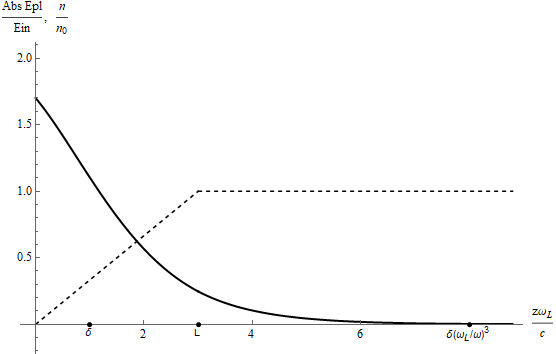
\includegraphics[scale=0.65]{mid_layer.png}}
	\caption{Зависимость абсолютного значения  поля внутри плазмы от расстояния до границы плазмы $z=0$.}
    \label{E_mid}
\end{figure}

Из выражения \eqref{coeff} получим коэффициент отражения в виде
\begin{equation}
    \label{coeff1_mid}
    R \approx \frac{\Gamma\left(1/3\right) - i\left(3c/\omega z_0\right)^{1/3}\Gamma\left(2/3\right)}{\Gamma\left(1/3\right) + i\left(3c/\omega z_0\right)^{1/3}\Gamma\left(2/3\right)}.
\end{equation}
Откуда следует, что коэффициент поглощения имеет вид 
\begin{equation}
    \label{coeff2_mid}
    A\left(\omega\right) \approx 4 \frac{\Gamma\left(1/3\right)}{3^{1/3}\Gamma\left(2/3\right)}\left(\frac{L\omega_L}{c}\right)^{1/3}\frac{\nu}{\omega_L}\left(1+\frac{\alpha}{3}\right).
\end{equation}
Сравнивая выражения \eqref{coeff2_small} и \eqref{coeff2_mid}, получаем, что в случае более широкого слоя переменной плотности коэффициент прохождения увеличивается в $\left(L\omega_L/c\right)^{1/3}$ раз в области частот падающего излучения, не близких к плазменной.
\subsection{Широкий слой}
Последний рассматриваемый случай имеет место, когда ширина слоя переменной плотности достаточно большая, а именно
\begin{equation}
    \label{cond3}
    \frac{\omega_L^3}{\omega^3}\frac{c}{\omega_L}<L.
\end{equation}

В этом случае абсолютные значения переменной $\xi$ на границах слоя $|\xi_0|, \, |\xi_L| \gg 1$. Учитывая значения $\arg \xi$, для границы $z=0$ воспользуемся выражениями \eqref{asymp_big_c} и \eqref{asymp_big_d}, а для $z=L$, как в предыдущем рассматриваемом случае, -- выражениями \eqref{asymp_big_a} и \eqref{asymp_big_b}. В данном случае, $\xi_L$ еще больше, чем в предыдущем разделе, поэтому можно положить коэффициент $C_2\approx 0$. Тогда поле внутри слоя имеет вид
\begin{equation}
  \label{E1_big}
  E\left(z\right) = 2E_0\sqrt{\pi}\left(\frac{\omega z_0}{c}\right)^{1/6}\exp\left[i\left(\frac{2}{3} \frac{\omega z_0}{c}-\frac{\pi}{4}\right)\right]Ai\left(\xi\left(z\right)\right).
\end{equation}
В области $z>L$, вычисляя коэффициент $C_3$ с учетом \eqref{E1_big}, получим
\begin{eqnarray}
    E\left(z\right) = E_0\left(\frac{1}{\gamma^2}\frac{\omega^2}{\omega_L^2-\omega^2}\right)^{1/4}\exp\left[-\frac{\sqrt{\omega_L^2-\omega^2}}{c}\gamma\left(z-L\right)+i\left(\frac{2}{3} \frac{\omega z_0}{c}-\frac{\pi}{4}\right)\right. \nonumber \\
    -\left.\frac{2}{3} \frac{\omega z_0}{c}\left(\gamma^2\frac{\omega_L^2-\omega^2}{\omega^2}\right)^{3/2}\right].
    \label{E2_big}
\end{eqnarray}
Учитывая \eqref{E1_big} и \eqref{E2_big}, поведение поля внутри плазмы сначала описывается периодической функцией, затем вблизи точки $L\omega^2/\omega_L^2$ убывающей линейно функцией и наконец затем экспоненциально убывающей функцией. Точное решение для абсолютного значения поля внутри плазмы $E\left(z\right)$ продемонстрировано на рис.\ref{E_big}. График на рисунке \ref{E_big} построен с использованием общих выражений \eqref{C1_common} и \eqref{C2_common} для параметров $\alpha = 4.8$, частоты падающего поля $\omega = 0.5\omega_L$, частоты столкновений фотоэлектронов $\nu = 0.01 \omega_L$ и ширины слоя $L = 15 c/\omega_L$. В этом случае, поле проникает еще глубже, чем в предущих рассматриваемых случаях. Однако затухание происходит еще до начала участка с постоянной плотностью фотоэлектронов.  
\begin{figure}[!ht]	
	\center{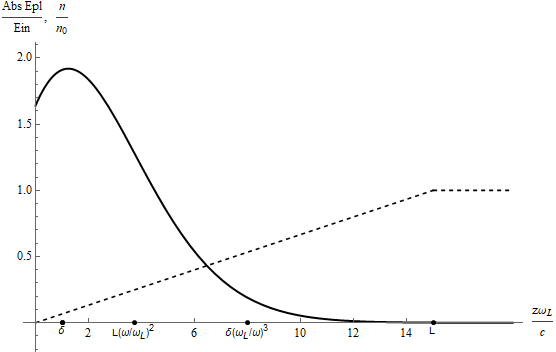
\includegraphics[scale=0.65]{thick_layer.png}}
	\caption{Зависимость абсолютного значения  поля внутри плазмы от расстояния до границы плазмы $z=0$.}
    \label{E_big}
\end{figure}

Коэффициент отражения в данном случае имеет вид 
\begin{equation}
    \label{coeff1_big}
    R = \exp\left[i\left(\frac{4}{3} \frac{\omega z_0}{c}-\frac{\pi}{2}\right)\right].
\end{equation}
Тогда для коэффициента поглощения имеем 
\begin{equation}
   \label{coeff2_big}
   A\left(\omega\right) = 1-\exp\left[-\frac{8}{3}\left(1+\alpha/3\right)\frac{\nu}{\omega_L}\frac{L\omega_L}{c}\frac{\omega^2}{\omega_L^2}\right].
\end{equation}
Таким образом, если $L\omega_L/c\cdot\omega^3/\omega_L^3\gg\omega/\nu$, то почти все поле поглощается плазмой, а в обратном случае поле почти целиком отражается.
\section{Нормальный скин-эффект}
Теперь рассмотрим обратное условие, когда $\nu \gg \omega$, отвечающее нормальному скин-эффекту. В этом случае функция $f\left(\omega, \nu, \alpha\right)$ имеет вид в линейном по $\omega/\nu$ приближении
\begin{equation}
    \label{f_ns}
    f\left(\omega, \nu, \alpha\right) \approx -\frac{1}{\nu^2}\left[i\left(1-\frac{\alpha}{3}\right)\frac{\nu}{\omega}+2\frac{\alpha}{3}-1+i\left(\alpha-1\right)\frac{\omega}{\nu}\right].
\end{equation}
Наличие дополнительного параметра $1-\alpha/3$ позволяет рассмотреть два различных случая. Если 
\begin{equation}
    \label{cond1}
    \nu\left(1-\frac{\alpha}{3}\right) \gg \omega,
\end{equation}
то выражение \eqref{f_ns} можно упростить до 
\begin{equation}
    \label{f_cond1}
    f\left(\omega, \nu, \alpha\right) \approx \frac{1}{i} \left(1-\frac{\alpha}{3}\right)\frac{1}{\nu\omega}.
\end{equation}
В условиях малости частоты столкновений и частоты падающего поля по сравнению с плазменной частотой $\sqrt{1-\alpha/3}\omega_L$ для корня из поперечной диэлектрической проницаемости имеем
\begin{equation}
    \label{perm_ns1}
    \sqrt{\varepsilon\left(\omega\right)} = \left(1+i\right)\frac{\omega_L}{\sqrt{\nu \omega}}\sqrt{\frac{1-\alpha/3}{2}}.
\end{equation}
Абсолютные значения $\xi_0$ и $\xi_L$ в данном случае имеют вид
\begin{equation}
\label{xi_ns1}
    |\xi_0|= \frac{1}{\omega_L^2}\left(\frac{\omega_L}{c}L\right)^{2/3}\left(\frac{\omega^2\nu}{1-\alpha/3}\right)^{2/3},\quad |\xi_L|\approx \left(\frac{\omega_L}{c}L\right)^{2/3}\left(\frac{\left(1-\alpha/3\right)\omega}{\nu}\right)^{1/3}.
\end{equation}
Из \eqref{xi_ns1} следует, что в условиях достаточно большой плазменной частоты $|\xi_l|>|\xi_0|$ и опять представляется возможным разделить все возможные ширины слоя переменной плотности фотоэлектронов на три части.
\subsection{Узкий слой}
Если ширина слоя удовлетворяет условию
\begin{equation}
    \label{thin_ns}
    L\frac{\omega_L}{c}< \left(\frac{\nu}{\left(1-\alpha/3\right)\omega}\right)^{1/2},
\end{equation}
тогда величины $|\xi_0|, |\xi_L| \ll 1$. Для получения поля внутри слоя переменной плотности воспользуемся \eqref{asymp_small} и получим
\begin{equation}
    \label{E1_ns_small}
    E\left(z\right)= 2E_0\frac{\left(L-z\right)\sqrt{\left(1-\alpha/3\right)\omega/\nu}+\left(i+1\right)c/\sqrt{2}\omega_L}{\left(L+ic/\omega\right)\sqrt{\left(1-\alpha/3\right)\omega/\nu}+\left(i+1\right)c/\sqrt{2}\omega_L}.
\end{equation}
В области $z>L$ поле имеет вид
\begin{equation}
    \label{E2_ns_small}
     E\left(z\right) = 2E_0   \frac{1}{\left[\left(1-i\right)\omega_L/\sqrt{2}c\right]\left(L+ic/\omega\right)\sqrt{\left(1-\alpha/3\right)\omega/\nu}+1}\exp\left[\frac{i-1}{\sqrt{2}}\sqrt{\left(1-\alpha/3\right)\frac{\omega}{\nu}}\frac{\omega_L}{c}\left(z-L\right)\right].
\end{equation}
Также, как и в случае высокочастотного скин-эффекта, поле внутри "узкого" слоя переменной плотности убывает линейно внутрь плазмы, а, когда плотность плазмы становится постоянной, медленно убывает экспоненциальным образом. Точное решение для абсолютного значения поля внутри плазмы $E\left(z\right)$ продемонстрировано на рис.\ref{E_small}. График на рисунке \ref{E_small} построен с использованием общих выражений \eqref{C1_common} и \eqref{C2_common} для параметров $\alpha = 2$, что соответствует плазме, полученной при ионизации ксенона со средней энергией фотоэлектронов $\epsilon_0\approx4.5\text{eV}$, частоты падающего поля $\omega = 0.05\omega_L$, частоты столкновений фотоэлектронов $\nu = 0.3 \omega_L$ и ширины слоя $L =2 c/\omega_L$. На оси $x$ обозначены характерные масштабы рассматриваемой задачи. Как видно из рисунка \eqref{E_small} поле внутрь плазмы проникает на расстояние порядка нескольких электромагнитных масштабов.
\begin{figure}[!ht]	
	\center{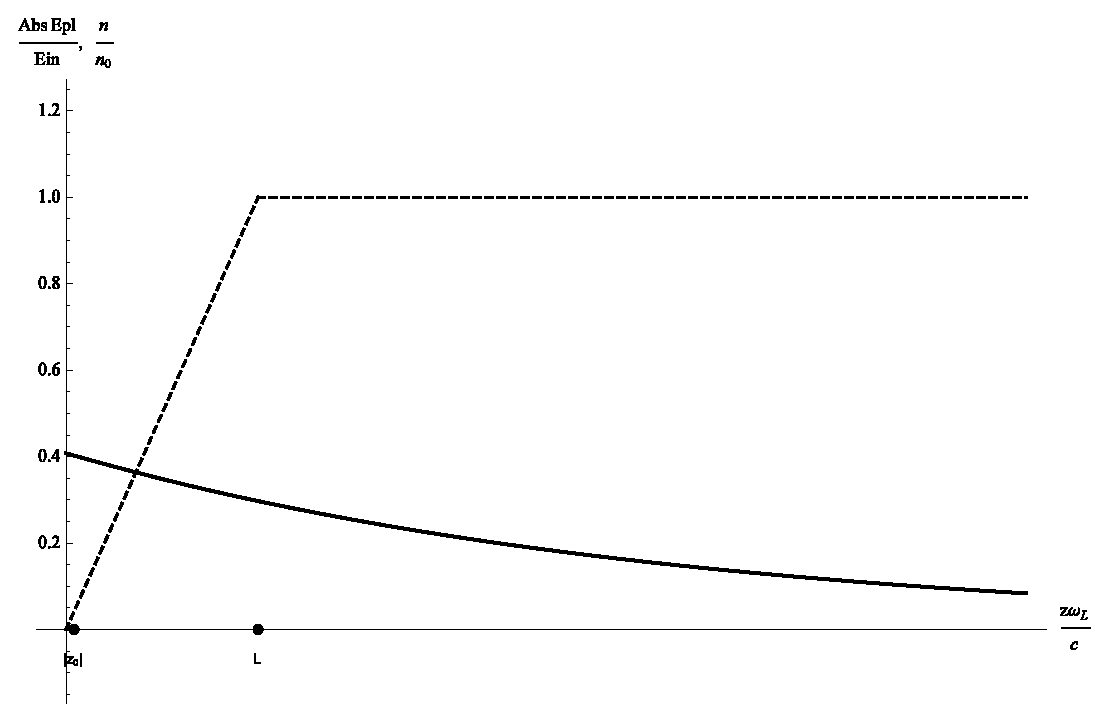
\includegraphics[scale=0.65]{ns_thin.eps}}
	\caption{Зависимость абсолютного значения  поля внутри плазмы от расстояния до границы плазмы $z=0$.}
    \label{E_small}
\end{figure}
Учитывая малость $\xi_0, \xi_L$ для коэффициента отражения получим
\begin{equation}
    \label{r_ns_thin}
    R = -\frac{\sqrt{\varepsilon\left(\omega\right)}-1}{\sqrt{\varepsilon\left(\omega\right)}+1},
\end{equation}
где $\sqrt{\varepsilon\left(\omega\right)}$ определено как \eqref{perm_ns1}. Тогда коэффициент поглощения в данном случае 
\begin{equation}
    \label{coeff_ns_thin}
    A(\omega)\approx  \sqrt{\frac{8\nu\omega}{\omega_L^2}}\frac{1}{\sqrt{1-\alpha/3}}.
\end{equation}
Этот же результат получается, если рассматривать плазму с резкой границей, то есть $L \to 0$ [ссылка на нашу работу].
\subsection{Промежуточная ширина слоя}
Рассмотрим случай, когда $|\xi_0|\ll 1$, а $|\xi_L| \gg 1$. Такие параметры соответсвуют ширине слоя переменной плотности в пределах 
\begin{equation}
    \label{cond2}
    \left(\frac{\nu}{\left(1-\alpha/3\right)\omega}\right)^{1/2}<L\frac{\omega_L}{c}<\frac{\omega_L^3}{\nu\omega^2}\left(1-\alpha/3\right).
\end{equation}
В этих условия $|\xi_L|\gg 1$ и поэтому основным слагаемым в знаменателе выражений \eqref{C1_common} и \eqref{C2_common}-то, в котором присутствует $Bi\left(\xi_L\right), Bi'\left(\xi_L\right)$. При этом с учетом асимптотики функции $Ai\left(\xi_L\right)$ в первом приближении $C_2=0$. Тогда для $0<z<L$ \begin{equation}
    \label{E1_ns_mid}
    E\left(z\right) = -2i E_0 3^{1/3} \Gamma\left(1/3\right)\left(\frac{\omega z_0}{c}\right)^{1/3} Ai\left(\xi\left(z\right)\right).
\end{equation} 
Внутри плазмы с постоянной плотностью фотоэлектронов
\begin{equation}
    \label{E2_ns_mid}
    E\left(z\right) \approx -iE_0 \frac{3^{1/3} \Gamma\left(1/3\right)}{\sqrt{\pi}}\left(\frac{\omega z_0}{c}\right)^{1/6}\left(\frac{z_0}{L}\right)^{1/4}
    \exp\left[\frac{i-1}{\sqrt{2}}\sqrt{\left(1-\alpha/3\right)\frac{\omega}{\nu}}\frac{\omega_L}{c}\left(z-L\right) - \frac{2}{3}\frac{\omega z_0}{c}\left(\frac{L}{z_0}\right)^{3/2}\right].
\end{equation}
Из выражения \eqref{coeff} получим коэффициент отражения в виде
\begin{equation}
    \label{coeff1_mid}
    R \approx \frac{\Gamma\left(1/3\right) - i\left(3c/\omega z_0\right)^{1/3}\Gamma\left(2/3\right)}{\Gamma\left(1/3\right) + i\left(3c/\omega z_0\right)^{1/3}\Gamma\left(2/3\right)}.
\end{equation}
Откуда следует, что коэффициент поглощения имеет вид 
\begin{equation}
    \label{coeff2_mid}
    A\left(\omega\right) \approx 2 \frac{\Gamma\left(1/3\right)}{3^{1/3}\Gamma\left(2/3\right)}\left(\frac{L\omega_L}{c} \frac{\nu\omega^2}{\omega_L^3\left(1-\alpha/3\right)}}\right)^{1/3}.
\end{equation}
\subsection{Широкий слой}
Если ширина слоя переменной плотности настолько велика, что выполнено условие
\begin{equation}
    \label{cond_ns_thick}
    L\frac{\omega_L}{c}>\frac{\omega_L^3}{\nu\omega^2}\left(1-\alpha/3\right),
\end{equation}
то величины $|\xi_0|, |\xi_L| \gg 1$. Тогда, воспользовавшись общими выражениями для коэффициентов \eqref{C1_common} и \eqref{C2_common}, а также асимптотикой функций Эйри, получим для $0<z<L$
\begin{equation}
  \label{E1_ns_big}
  E\left(z\right) = 2E_0\sqrt{\pi}\left(\frac{\omega z_0}{c}\right)^{1/6}\exp\left[i\left(\frac{2}{3} \frac{\omega z_0}{c}-\frac{\pi}{4}\right)\right]Ai\left(\xi\left(z\right)\right).
\end{equation}
(такое же, как в предыдущем случае высокочастотного скин-эффекта).
Отличаться будет коэффициент поглощения 
\begin{equation}
\label{coeff_ns_big}
       A\left(\omega\right) = 1-\exp\left[-\frac{8}{3}\frac{\nu\omega^2}{\omega_L^3\left(1-\alpha/3\right)}\frac{L\omega_L}{c}\right].
\end{equation}
\section{Диэлектрик}
Если помимо условия $\nu\gg\omega$ выполнено условие 
\begin{equation}
    \label{cond2}
    \nu\left(1-\frac{\alpha}{3}\right)\ll\omega,
\end{equation}
то основным в выражении \eqref{f_ns} будет действительное слагаемое. Такой режим легко реализуем при значении $\alpha\approx 3$. Поперечную диэлектрическую проницаемость внутри слоя переменной плотности можно записать в виде 
\begin{equation}
    \label{perm_diel}
    \varepsilon\left(\omega, z\right) \approx 1 + \frac{z}{L}\frac{\omega_L^2}{\nu^2}\left[2\frac{\alpha}{3}-1+i\left(\alpha-1\right)\frac{\omega}{\nu}\right] = 1 + \frac{z}{L}\left(\varepsilon'_L+i\varepsilon_L''\right)
\end{equation}
где $\varepsilon'_L \gg \varepsilon''_L$. Учитывая аналитические свойства функции Эйри $\xi$ и вид поперечной диэлектрической проницаемости в точке $z=L$, замена в уравнении \eqref{field2} в данном случае имеет вид
\begin{equation}
    \label{xi_diel}
    \xi = -\left(\frac{\omega^2}{z_0c^2}\right)^{1/3}\left(z+z_0\right),
\end{equation}
где $z_0=L/\left(\varepsilon'_L+i\varepsilon_L''\right)$. При этом в точках $z=0$ и $z=L$ справедливы оценки
\begin{equation}
\label{xi_diel}
    |\xi_0| \approx \left(\frac{\omega_L L}{c}\frac{\omega\nu^2}{\omega_L^3\left(2\alpha/3-1\right)}\right)^{2/3}, \quad |\xi_L| \approx  \left(\frac{\omega_L L}{c}\right)^{2/3}\left(\frac{\omega^2}{\nu^2}\left(2\frac{\alpha}{3}-1\right)\right)^{1/3}.
\end{equation}
\subsection{Узкий слой}
Если 
\begin{equation}
    \label{thin_diel}
    L\frac{\omega_L}{c}<\frac{\nu}{\omega\sqrt{2\alpha/3-1}},
\end{equation}
то значения \eqref{xi_diel} малы, а значит можно воспользоваться асимптотикой функций Эйри \eqref{asymp_small}. Тогда для $0<z<L$ получим
\begin{equation}
    \label{E1_diel_small}
    E\left(z\right)\approx 2E_0 \frac{i\left(L-z\right)\sqrt{2\alpha/3-1}\omega\omega_L/c\nu+1}{i\left(L+ic/\omega\right)\sqrt{2\alpha/3-1}\omega\omega_L/c\nu+1}
\end{equation}
В области $z>L$ поле имеет вид
\begin{equation}
    \label{E2_diel_small}
     E\left(z\right) \approx 2E_0   \frac{1}{i\left(L+ic/\omega\right)\sqrt{2\alpha/3-1}\omega\omega_L/c\nu+1}\exp\left[i\frac{\omega}{c}\sqrt{\varepsilon}\left(z-L\right)\right],
\end{equation}
где $\sqrt{\varepsilon}$ имеет вид \eqref{perm_diel}. Коэффициент отражения определяется таким же выражением, как и \eqref{r_ns_thin}, а коэффициент поглощения в данном случае имеет вид
\begin{equation}
    \label{a_diel_thin}
    A\left(\omega\right) \approx 4\frac{\nu}{\omega_L}\frac{1}{\sqrt{2\alpha/3-1}}.
\end{equation}
\subsection{Слой промежуточной ширины}
Если же ширина слоя удовлетворяет условию 
\begin{equation}
    \label{diel_mid}
    \frac{\nu}{\omega\sqrt{2\alpha/3-1}}<L\frac{\omega_L}{c}<\frac{\omega_L^3}{\omega\nu^2}\left(2\alpha/3-1\right),
\end{equation}
то выполняются условия $|\xi_0|\ll 1$, а $|\xi_L|\gg 1$. Тогда, воспользовавшись \eqref{asymp_big} и \eqref{asymp_small} получим внутри слоя переменной плотности фотоэлектронов 
\begin{equation}
    \label{E1_diel_mid}
    E\left(z\right) \approx \frac{2E_0}{\left(\sqrt{3}+i\right)\Tilde{C_1}+\left(c/\omega z_0\right)^{1/3}\left(1+\sqrt{3}i\right)\Tilde{C_2}}\left[iAi\left(\xi\right)+Bi\left(\xi\right)\right],
\end{equation}
где $\Tilde{C_1} = (3^{2/3}\Gamma(2/3))^{-1},\Tilde{C_2} = (3^{1/3}\Gamma(1/3))^{-1}$ - коэффициенты из асимптотики функций Эйри для малых аргументов \eqref{asymp_small}. 
Для $z>L$ поле имеет вид
\begin{eqnarray}
    E\left(z\right) \approx \frac{2E_0}{\varepsilon^{1/4}\sqrt{\pi}}\left(\frac{\omega z_0}{c}\right)^{1/6}\frac{1}{\left(\sqrt{3}+i\right)\left(\omega z_0/c\right)^{1/3}\Tilde{C_1}+\left(1+\sqrt{3}i\right)\Tilde{C_2}} \nonumber \\
    \exp\left[i\left(\frac{\omega}{c}\sqrt{\varepsilon}\left(z-L\right)+\frac{2}{3}\frac{\omega z_0}{c}\varepsilon^{3/2}+\frac{\pi}{4}\right)\right],
\label{E2_diel_mid}
\end{eqnarray}
Коэффициент поглощения в данном случае имеет вид
\begin{equation}
    \label{a_diel_mid}
    A\left(\omega\right) \approx 3^{1/6}\frac{\Gamma(1/3)}{\Gamma(2/3)}\left(\frac{L\omega_L}{c}\frac{\nu^2\omega}{\omega_L^3}\right)^{1/3}.
\end{equation}
\subsection{Широкий слой диэлектрика}
Когда ширина слоя переменной плотности достаточно велика
\begin{equation}
    \label{diel_thick}
    L\frac{\omega_L}{c}>\frac{\omega_L^3}{\omega\nu^2}\left(2\alpha/3-1\right),
\end{equation}
то $|\xi_0|\gg 1$ и $|\xi_L|\gg 1$. Воспользовавшись асимптотикой \eqref{asymp_big} получим поле внутри слоя переменной плотности в виде
\begin{equation}
\label{E1_diel_thick}
    E\left(z\right) \approx E_0 \left(\frac{z_0}{z+z_0}\right)^{1/4} \exp\left[\frac{2}{3}i\left((-\xi)^{3/2}-(-\xi_0)^{3/2}\right)\right].
\end{equation}
Для области $z>L$ поле имеет вид
\begin{equation}
\label{E2_diel_thick}
E\left(z\right) = \frac{E_0}{\varepsilon^{1/4}}\exp\left[i\frac{\omega}{c}\sqrt{\varepsilon}\left(z-L\right)+\frac{2}{3}i\frac{\omega z_0}{c}\left(\varepsilon^{3/2}-1\right)\right].
\end{equation}
Коэффициент поглощения в данном случае
\begin{equation}
    A\left(\omega\right) \approx 1.
\end{equation}
\end{document}
